% =====================================================================
% Application paper -- AAAI-style draft
% BUILD: tools/tectonic/tectonic.exe docs/aaai_bruise_paper.tex
% NOTE: AAAI ships aaai26.sty via its author kit (not CTAN), so it is
% not fetchable by the Tectonic build used here. The preamble below
% reproduces the AAAI two-column 10pt layout closely for drafting.
% Replace the block between AAAI-STYLE markers with the official
% aaai26.sty/aaai26.bst before submission.
% =====================================================================
\documentclass[letterpaper,twocolumn,10pt]{article}

% ---------------- AAAI-STYLE BLOCK (replace with aaai26.sty) ----------
\usepackage[letterpaper, top=0.75in, bottom=1.0in,
            left=0.75in, right=0.75in, columnsep=0.25in]{geometry}
\usepackage{times}
\usepackage{helvet}
\usepackage{courier}
\renewcommand{\familydefault}{\rmdefault}
\pagestyle{empty}
% ---------------- END AAAI-STYLE BLOCK -------------------------------

\usepackage[T1]{fontenc}
\usepackage[utf8]{inputenc}
\usepackage{amsmath,amssymb}
\usepackage{graphicx}
\usepackage{booktabs}
\usepackage{array}
\usepackage{caption}
\usepackage{url}
\usepackage{pgfplots}
\pgfplotsset{compat=1.17}
\usepackage[hidelinks]{hyperref}

\setlength{\parskip}{0pt}
\setlength{\abovecaptionskip}{4pt}
\captionsetup{font=small,labelfont=bf}
\newcommand{\dice}{\mathrm{Dice}}

\title{\bf The Annotation Ceiling in Forensic Bruise Segmentation:\\
When a Model Agrees with Expert Consensus Better Than the Expert It Learned From}
\author{Anonymous Submission}
\date{}

\begin{document}
\maketitle

\begin{abstract}
White-light photography of bruises is central to forensic injury documentation,
yet automatic bruise segmentation is trained and evaluated against annotations
that expert clinicians themselves disagree about. We study this problem on the
NIJ white-light bruise corpus under a deliberately strict, application-faithful
protocol: models are trained on a single expert's masks and evaluated on the
\emph{2-of-3 majority consensus} of the three highest-volume annotators, over the
185-image / 28-subject strict intersection that all three labeled. Under this
cross-annotator generalization test we make three contributions. First, we
measure the \emph{annotation ceiling}: the three experts agree with one another at
only $0.639$ mean Dice, well below the agreement between our models and the
consensus target. Second, and counterintuitively, a compact SegFormer-B0 trained
\emph{only} on one annotator (Paul) agrees with the three-expert consensus
significantly better than that annotator does himself (mean Dice
$+0.067$, subject-level cluster-bootstrap $95\%$ CI $[+0.003,+0.133]$): training
averages away an annotator's idiosyncrasies and keeps what generalizes. Third, in
a controlled comparison of seven architectures (SegFormer-B2/B0, YOLO26n-sem,
U-Net, DeepLabV3+) trained under one recipe, every capable model clusters in a
narrow $0.74$--$0.77$ mean-Dice band; the differences that \emph{are} resolvable
at this consensus-limited sample size live in failure rates and cross-seed
stability, not in headline Dice, and distillation is statistically
indistinguishable from its baseline. Our results reframe ``underpowered'' from an
apology into a mechanism: forensic bruise segmentation is \emph{label-limited, not
capacity-limited}, and the field's binding constraint is annotation consensus, not
model architecture.
\end{abstract}

\section{Introduction}
Bruises are among the most common findings in cases of interpersonal violence,
elder abuse, and child maltreatment, and their photographic documentation carries
evidentiary weight. Automatic segmentation of the bruised region from a clinical
photograph promises consistent, reproducible documentation. In practice, however,
the ``ground truth'' used to train and score such systems is produced by human
annotators whose delineations disagree substantially, because the boundary of a
bruise is genuinely ambiguous: it fades gradually into normal skin and its
apparent extent depends on lighting, body site, and the rater. This makes bruise
segmentation an unusually honest testbed for a question that pervades applied
medical imaging but is rarely confronted directly: \emph{what can a segmentation
benchmark actually tell us when the labels themselves are noisy and the
consensus-labeled test set is necessarily small?}

We approach this as an application study on the NIJ white-light bruise corpus. Our
design is driven by two facts about the data. (i) The corpus was labeled by many
annotators; only the three highest-volume annotators (denoted Paul, Gbarimah,
Erik) share enough images to define a common evaluation set. Their strict
intersection is \textbf{185 images from 28 subjects}. (ii) There is no way to
enlarge this consensus set without commissioning new expert annotation: $n=28$
subjects is a \emph{ceiling imposed by the availability of three-annotator
consensus labels}, not a design choice. We therefore treat the majority vote of
the three experts as the test target, train on the non-intersection images of a
single, previously-selected best annotator (Paul), and evaluate every model as a
\emph{cross-annotator generalization} problem: how well does a model trained on one
expert reproduce the consensus of three?

Within this protocol we compare seven segmentation models spanning three
families---a semantic transformer (SegFormer-B2/B0), a detector-derived semantic
head (YOLO26n-sem), and two classic encoder--decoder CNNs (U-Net, DeepLabV3+)---all
trained under one shared recipe so that architecture is the isolated variable.
Rather than crown a winner, we ask which conclusions survive the statistical
reality of a 28-subject consensus test set, using subject-level cluster
bootstrapping throughout.

\paragraph{Contributions.}
\begin{itemize}\itemsep2pt
\item An application-faithful, multi-annotator evaluation protocol for white-light
bruise segmentation: train on one expert, test on three-expert majority consensus
over the strict labeled intersection, with subject-disjoint splits.
\item A quantified \emph{annotation ceiling}: expert--expert agreement ($0.639$
mean Dice) is lower than model--consensus agreement, establishing that the models
are label-limited.
\item The main empirical finding: a model trained on a single annotator agrees
with the three-expert consensus \emph{significantly better than that annotator
himself} (mean Dice $+0.067$, $95\%$ CI $[+0.003,+0.133]$). To our knowledge this
``model-beats-its-annotator'' effect has not been reported for forensic imaging.
\item A controlled seven-architecture comparison showing convergence at the
ceiling: capable models differ in failure rate and stability, not headline Dice,
and knowledge distillation is not resolvable from zero at this sample size.
\end{itemize}

\section{Related Work}
\paragraph{Medical and forensic image segmentation.}
Encoder--decoder CNNs (U-Net~\cite{unet}, DeepLabV3+~\cite{deeplabv3plus}) and their
self-configuring descendants (nnU-Net~\cite{nnunet}) remain the default for
biomedical segmentation, while transformer segmenters such as
SegFormer~\cite{segformer} have become strong, efficient alternatives. Recent
one-stage detectors expose semantic-segmentation heads (e.g.,
YOLO26~\cite{yolo26}), enabling real-time masks. Forensic bruise imaging has
historically focused on \emph{visibility} rather than automatic delineation, with
alternate-light and cross-polarized techniques studied for enhancing bruise
contrast~\cite{scafide}. We contribute an application study that segments bruises
on standard white-light photographs and, critically, evaluates against a
multi-expert consensus rather than a single rater.

\paragraph{Label noise and inter-observer variability.}
That expert annotations disagree is well documented in medical
imaging~\cite{joskowicz,warfield}, and consensus-fusion methods such as
STAPLE~\cite{warfield} estimate a hidden ``true'' segmentation from multiple
raters. Our aim is different: we use the observed multi-rater disagreement as a
\emph{measuring stick}---an annotation ceiling---and quantify how model--consensus
agreement compares to expert--consensus agreement. The finding that a model can
match consensus better than an individual rater is related to the ``wisdom of
crowds'' rationale behind label fusion, but we show it emerges from
\emph{single-annotator} training via generalization, not from fusing raters.

\paragraph{Knowledge distillation.}
Knowledge distillation~\cite{hinton} transfers a large teacher's soft predictions
to a compact student and is widely used to shrink segmentation models. We evaluate
it here as one of the interventions whose effect we test for statistical
resolvability at forensic sample sizes.

\paragraph{Uncertainty at small sample sizes.}
When test images are clustered within few subjects, the effective sample size is
the number of subjects, and subject-level (cluster) resampling is required for
valid inference~\cite{clusterboot}. We adopt paired subject-level cluster
bootstrapping for all model comparisons, which is both correct for a shared test
set and tighter than independent resampling.

\section{Dataset and Multi-Annotator Design}
\paragraph{Corpus and consensus set.}
We use the NIJ white-light bruise corpus. Among its annotators, the three with the
largest labeled volume (Paul, Gbarimah, Erik) share a common set of images; their
\textbf{strict intersection is 185 white-light images from 28 subjects}, which we
fix as the test set. The test target is the \textbf{2-of-3 pixel majority vote} of
the three experts---a pixel is positive iff at least two of the three annotators
marked it positive.

\paragraph{Training data and disjointness.}
A prior five-fold cross-annotator study selected Paul as the most stable annotator
for training. All models are therefore trained on Paul's \emph{non-intersection}
images (697 train / 134 validation), which are \emph{subject-disjoint} from the 28
test subjects by construction. Evaluating a Paul-trained model against the
three-expert majority is thus a genuine cross-annotator generalization test, not a
within-distribution split.

\paragraph{The $n=28$ ceiling.}
There are 28 test subjects because that is how many subjects all three experts
annotated; a 29th requires new expert annotation. This reframes every
``underpowered'' result: it is not that our study is too small, but that
\emph{at the maximum size for which three-annotator consensus exists,
model-level differences are unresolvable}---a statement about the field, not the
experiment.

\section{Methods}
\paragraph{Preprocessing.}
Every image and mask is resized once to a common $640{\times}640$ grid (bilinear
for images, nearest for masks) so that prediction and ground truth are compared on
one grid and no mask is ever resized to match another. Pixels are scaled to
$[0,1]$; the ImageNet normalization each backbone expects is applied inside the
model, so a single neutral data pipeline feeds all architectures.

\paragraph{Architectures.}
We evaluate: SegFormer-B2 (teacher) and SegFormer-B0 (student) transformer
segmenters; the YOLO26n semantic-segmentation head (YOLO26n-sem); and U-Net and
DeepLabV3+ with ResNet-50 encoders as classic baselines. Parameter counts span
$1.6$M--$32.5$M (Table~\ref{tab:main}).

\paragraph{Training recipe.}
All non-detector models share one recipe: Dice$+$BCE loss, AdamW with a separate
(lower) learning rate for the pretrained encoder and a $10{\times}$ rate for the
randomly initialized decoder, no weight decay on norm/bias parameters, linear
warmup then polynomial decay, and early stopping on validation. YOLO26n-sem is
trained with its native detector pipeline (its own letterbox preprocessing,
augmentation, and schedule), and evaluated with its native argmax decision, which
is how it was designed to run. SegFormer models are trained with three seeds;
U-Net/DeepLabV3+ baselines with a single seed (a stated limitation).

\paragraph{Knowledge distillation.}
For the distilled variants, the SegFormer-B0 student is trained with an additional
term matching the SegFormer-B2 teacher's soft outputs; the YOLO distilled variant
uses offline teacher pseudo-masks. Distillation weights follow the project's
tuned values.

\paragraph{Operating point.}
A model emits a per-pixel score; a binary mask requires a threshold. For each
model we sweep the decision threshold \emph{on the validation set only} and apply
the chosen value once to the test set. Thresholding a monotone score is equivalent
to thresholding the raw logit, so the choice is a single one-dimensional cut and
never touches the test data.

\paragraph{Metrics and inference.}
We report per-image Dice and IoU, and---separately---the \emph{complete-miss rate}:
the fraction of images that contain a bruise but for which the model predicts no
positive pixels. A blank mask is a missed injury and is far worse than a loose
outline, so it is reported on its own. Because per-image Dice is strongly bimodal
(a model either localizes the bruise or misses it), we emphasize the median and
use percentile bootstraps rather than normal-theory intervals. All comparisons use
paired, subject-level cluster bootstrapping ($B{=}4000$ over the 28 subjects).

\section{Results}

\begin{table*}[t]
\centering
\small
\caption{Test performance on the 185-image / 28-subject consensus set (majority
target, scored at $640{\times}640$). SegFormer/YOLO are mean$\pm$std over three
seeds (YOLO uses native argmax); U-Net/DeepLabV3+ are single-seed ($\dagger$).
Speed is single-frame latency on an A100. Every capable model falls in a narrow
$0.74$--$0.77$ mean-Dice band; the spread is in complete-miss rate and stability.}
\label{tab:main}
\begin{tabular}{lccccc}
\toprule
Model & Params (M) & Mean Dice & Median Dice & Complete-miss (\%) & FPS (A100) \\
\midrule
SegFormer-B2 (teacher)      & 27.3 & $0.765\pm0.004$ & 0.811 & \textbf{0.00} & 29.7 \\
SegFormer-B0 (direct)       & 3.7  & $0.760\pm0.006$ & 0.811 & 0.54 & 60.0 \\
SegFormer-B0 (distilled)    & 3.7  & $0.764\pm0.005$ & 0.811 & 0.18 & 60.1 \\
U-Net (ResNet-50)$^{\dagger}$      & 32.5 & 0.741 & \textbf{0.828} & 5.41 & --- \\
DeepLabV3+ (ResNet-50)$^{\dagger}$ & 26.7 & 0.736 & 0.800 & 2.16 & --- \\
YOLO26n-sem (direct)        & \textbf{1.6}  & $0.691\pm0.020$ & 0.802 & 7.57 & \textbf{122.2} \\
YOLO26n-sem (distilled)     & 1.6  & $0.668\pm0.065$ & 0.766 & 7.57 & 121.7 \\
\bottomrule
\end{tabular}
\end{table*}

\paragraph{The models cluster; the winner depends on the metric.}
Table~\ref{tab:main} summarizes test performance. The three SegFormer variants and
the two classic CNN baselines all sit within a $0.74$--$0.77$ mean-Dice band and a
$0.80$--$0.83$ median-Dice band. Strikingly, the \emph{highest median Dice}
($0.828$) belongs to U-Net, whose complete-miss rate ($5.4\%$) is an order of
magnitude worse than SegFormer's ($\leq 0.5\%$): the best-Dice model is not the
safest model. The compact SegFormer-B0 ($3.7$M parameters) matches or beats both
classic baselines ($32.5$M, $26.7$M) at roughly one-eighth the parameters and near-zero
miss rate---a clean accuracy/efficiency result. YOLO26n-sem is the fastest by far
($122$ FPS) but the least accurate and, importantly, the least stable
(cross-seed std up to $0.065$ vs.\ $\leq0.006$ for SegFormer), with one distilled
seed collapsing entirely.

\paragraph{Distillation is not resolvable from zero.}
The distilled SegFormer-B0 improves mean Dice by only $+0.004$ over its direct
counterpart---smaller than the $\pm0.005$ cross-seed standard deviation---and a
paired subject-level cluster bootstrap does not separate the effect from zero. For
YOLO, distillation \emph{hurts} (mean $0.668$ vs.\ $0.691$) and inflates variance.
At this consensus-limited sample size, distillation is a wash.

\paragraph{Efficiency--accuracy trade-off.}
Figure~\ref{fig:pareto} plots mean Dice against parameter count. SegFormer-B0
dominates the classic baselines (higher Dice, $\sim9\times$ fewer parameters); the
teacher buys no measurable accuracy over the distilled student; YOLO trades a
large accuracy and safety penalty for throughput.

\begin{figure}[t]
\centering
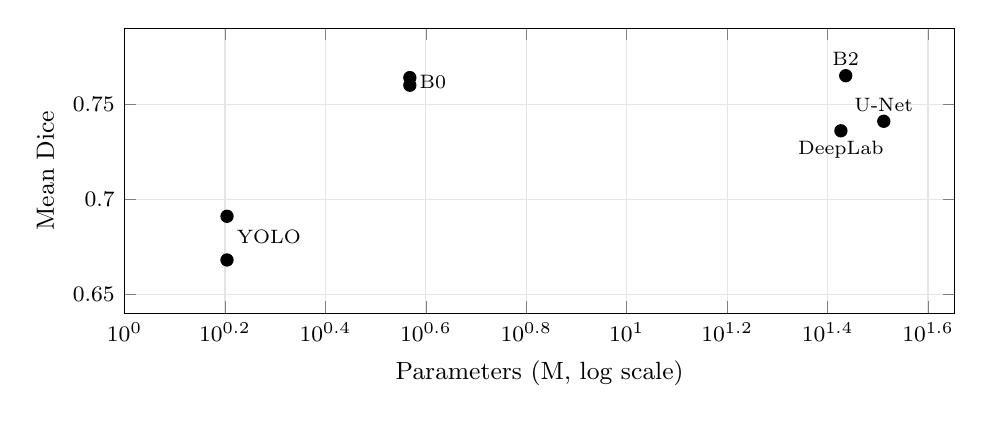
\begin{tikzpicture}
\begin{axis}[
  width=\columnwidth, height=5.2cm,
  xlabel={Parameters (M, log scale)}, ylabel={Mean Dice},
  xmode=log, log basis x=10,
  xmin=1, xmax=45, ymin=0.64, ymax=0.79,
  grid=both, grid style={gray!20},
  tick label style={font=\footnotesize}, label style={font=\small},
  scatter/classes={a={mark=*,draw=black}},
]
\addplot[only marks, mark=*, mark size=2.2pt] coordinates {
 (27.3,0.765) (3.7,0.760) (3.7,0.764) (32.5,0.741) (26.7,0.736) (1.6,0.691) (1.6,0.668)
};
\node[font=\scriptsize,anchor=south] at (axis cs:27.3,0.765) {B2};
\node[font=\scriptsize,anchor=west]  at (axis cs:3.7,0.762)  {B0};
\node[font=\scriptsize,anchor=south] at (axis cs:32.5,0.741) {U-Net};
\node[font=\scriptsize,anchor=north] at (axis cs:26.7,0.736) {DeepLab};
\node[font=\scriptsize,anchor=west]  at (axis cs:1.6,0.680)  {YOLO};
\end{axis}
\end{tikzpicture}
\caption{Accuracy vs.\ model size. SegFormer-B0 ($3.7$M) sits on the accuracy
frontier, matching the $\sim9\times$ larger classic baselines.}
\label{fig:pareto}
\end{figure}

\section{The Annotation Ceiling}
\paragraph{The experts barely agree with each other.}
Table~\ref{tab:inter} reports pairwise inter-annotator Dice on the 185 consensus
images, computed by pure mask arithmetic (no model). The three experts agree with
one another at only $0.639$ mean Dice on average. Every capable model in
Table~\ref{tab:main} agrees with the majority target \emph{better} than the
experts agree with each other. The labels are noisier than the models.

\begin{table}[t]
\centering
\small
\caption{Inter-annotator agreement on the 185 consensus images. The three experts
agree with each other far less ($0.639$ mean) than models agree with the majority
target. Paul---the annotator we train on---agrees with the majority \emph{least} of
the three.}
\label{tab:inter}
\begin{tabular}{lcc}
\toprule
Comparison & Mean Dice & Median Dice \\
\midrule
Gbarimah $\leftrightarrow$ Erik      & 0.755 & 0.809 \\
Paul $\leftrightarrow$ Gbarimah      & 0.581 & 0.633 \\
Paul $\leftrightarrow$ Erik          & 0.581 & 0.616 \\
\textbf{Avg.\ human--human}          & \textbf{0.639} & --- \\
\midrule
Gbarimah vs.\ majority               & 0.873 & 0.926 \\
Erik vs.\ majority                   & 0.866 & 0.892 \\
\textbf{Paul vs.\ majority}          & \textbf{0.700} & 0.750 \\
\bottomrule
\end{tabular}
\end{table}

\paragraph{Paul is the outlier we train on.}
Gbarimah and Erik agree with each other most ($0.755$), so the majority vote is
effectively ``what Gbarimah and Erik agreed on.'' Paul---whose masks we train
on---matches that target \emph{least} of the three ($0.700$ vs.\ $0.873$, $0.866$).
This does not contradict Paul's selection for training, which was based on the
downstream generalization of a Paul-trained model, a different criterion from
agreeing with peers.

\paragraph{Main result: the model beats the annotator it learned from.}
We compare the val-selected SegFormer-B0 (distilled) against Paul, both scored
against the same three-expert majority, with a paired subject-level cluster
bootstrap ($B{=}4000$, 28 subjects). The model agrees with the consensus
significantly better than Paul does:
{\small
\[
\begin{aligned}
\Delta_{\text{mean}} &= +0.067,\ \text{CI}\,[+0.003,+0.133],\ P(\Delta{>}0){=}98.0\%,\\
\Delta_{\text{median}} &= +0.063,\ \text{CI}\,[-0.002,+0.129],\ P(\Delta{>}0){=}96.9\%.
\end{aligned}
\]}%
(all Dice; $95\%$ subject-level cluster-bootstrap CIs.)
A model trained \emph{only} on Paul's masks reproduces the three-expert consensus
better than Paul himself: training averages away one annotator's idiosyncrasies
and retains what generalizes. For scale, this effect is an order of magnitude
larger than---and unlike---the distillation effect ($+0.004$, n.s.) that a
conventional benchmark would have foregrounded.

\paragraph{Why this explains the null model comparisons.}
We were attempting to resolve $\sim0.02$-Dice architecture differences against a
target that carries roughly $0.36$ of annotation noise ($1-0.639$). That was never
going to resolve. The models are label-limited, not capacity-limited; the
architecture ranking is inside the noise floor, while the label-versus-model gap
is not.

\section{Discussion}
Our results invert the usual reading of a flat leaderboard. The convergence of
five capable architectures into a narrow Dice band is not a failure to find a
better model; it is evidence that model capacity is no longer the binding
constraint for this task at its current label quality. Two consequences follow for
practitioners. First, \emph{report failure rates and cluster-level intervals, not
just mean Dice}: complete-miss rate cleanly separates the models
($0$--$0.5\%$ for SegFormer, $2.2\%$ for DeepLabV3+, $5.4\%$ for U-Net, $7.6\%$ for
YOLO) where Dice does not, and it is the clinically decisive quantity. Second,
\emph{invest in annotation, not architecture}: at $28$ subjects the minimum
resolvable median-Dice effect is $\sim0.04$, larger than the gaps between
transformer, CNN, and detector families, so further architecture search on this
target buys unmeasurable gains, whereas additional consensus annotation directly
raises the ceiling. The ``model beats its annotator'' effect suggests a concrete
path: models trained on individual raters can serve as consensus-approximating
pre-labelers to accelerate the very annotation the field is short of.

\section{Limitations}
The consensus test set is fixed at $28$ subjects; this is a ceiling, but it bounds
statistical power and we do not claim architecture rankings beyond it. The
U-Net/DeepLabV3+ baselines are single-seed and used a marginally different
train/validation partition (identical test set), so their point estimates lack the
seed error bars of the transformer models; a matched multi-seed re-run is planned.
YOLO is trained and scored in its native pipeline rather than the shared recipe,
which is the fair choice for a detector but means its numbers reflect a different
preprocessing chain. Intervals capture test-set sampling only, not training
stochasticity, so they are, if anything, optimistic. Finally, we deliberately omit
skin-tone subgroup (fairness) analysis: the worst-group Dice gap is an
extremum-of-extrema statistic whose subject-level cluster-bootstrap interval at
this sample size is too wide to support a claim, and reporting it as a finding
would repeat exactly the over-interpretation this paper cautions against.

\section{Conclusion}
On a strict, multi-annotator forensic bruise benchmark we show that expert
annotators agree with one another less than our models agree with their consensus,
and that a compact model trained on a single annotator reproduces three-expert
consensus significantly better than that annotator himself. Across seven
architectures, headline Dice is unresolvable at the consensus-limited sample size,
while failure rate and stability are not. Forensic bruise segmentation is
label-limited: the path forward is more consensus annotation and honest,
cluster-level reporting---not a larger model.

\begin{thebibliography}{99}
\small
\bibitem{segformer} E.~Xie, W.~Wang, Z.~Yu, A.~Anandkumar, J.~M. Alvarez, and P.~Luo.
SegFormer: Simple and Efficient Design for Semantic Segmentation with Transformers.
\emph{NeurIPS}, 2021.
\bibitem{unet} O.~Ronneberger, P.~Fischer, and T.~Brox.
U-Net: Convolutional Networks for Biomedical Image Segmentation. \emph{MICCAI}, 2015.
\bibitem{deeplabv3plus} L.-C. Chen, Y.~Zhu, G.~Papandreou, F.~Schroff, and H.~Adam.
Encoder-Decoder with Atrous Separable Convolution for Semantic Image Segmentation
(DeepLabV3+). \emph{ECCV}, 2018.
\bibitem{nnunet} F.~Isensee, P.~F. Jaeger, S.~A.~A. Kohl, J.~Petersen, and K.~H. Maier-Hein.
nnU-Net: A Self-Configuring Method for Deep Learning-Based Biomedical Image
Segmentation. \emph{Nature Methods}, 18(2):203--211, 2021.
\bibitem{yolo26} G.~Jocher et al. YOLO26: Real-Time End-to-End Object Detection and
Segmentation. \emph{arXiv:2606.03748}, 2026.
\bibitem{hinton} G.~Hinton, O.~Vinyals, and J.~Dean.
Distilling the Knowledge in a Neural Network. \emph{NeurIPS Deep Learning Workshop}, 2015.
\bibitem{warfield} S.~K. Warfield, K.~H. Zou, and W.~M. Wells.
Simultaneous Truth and Performance Level Estimation (STAPLE): An Algorithm for the
Validation of Image Segmentation. \emph{IEEE TMI}, 23(7):903--921, 2004.
\bibitem{joskowicz} L.~Joskowicz, D.~Cohen, N.~Caplan, and J.~Sosna.
Inter-Observer Variability of Manual Contour Delineation of Structures in CT.
\emph{European Radiology}, 29(3):1391--1399, 2019.
\bibitem{scafide} K.~N. Scafide, D.~J. Sheridan, J.~Taylor, and M.~E. Hayat.
Detection of Inflicted Bruises by Alternate Light: Results of a Randomized
Controlled Trial. \emph{Journal of Forensic Sciences}, 65(4):1191--1198, 2020.
\bibitem{clusterboot} C.~A. Field and A.~H. Welsh.
Bootstrapping Clustered Data. \emph{Journal of the Royal Statistical Society: Series B},
69(3):369--390, 2007.
\bibitem{milletari} F.~Milletari, N.~Navab, and S.-A. Ahmadi.
V-Net: Fully Convolutional Neural Networks for Volumetric Medical Image
Segmentation. \emph{3DV}, 2016.
\end{thebibliography}

\end{document}
